   %\begin{wrapfigure}{l}{0.4\textwidth}          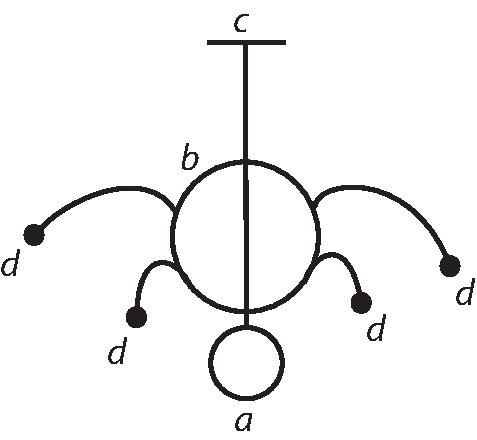
\includegraphics[width=0.4\textwidth]{images/35_15_6_48v1}
   %\end{wrapfigure}
[48 r\textsuperscript{o}] Si navis\protect\index{Sachverzeichnis}{navis} quiescat deberet eidem puncto infigi acus\protect\index{Sachverzeichnis}{acus}, ac ita non poterunt numerari horae. Similiter fieri possit ut \edtext{situs}{\lemma{ut}\Afootnote{ \textit{ (1) }\ acus \textit{ (2) }\ situs \textit{ L}}} punctorum sit \textit{a} ubi motus navis\protect\index{Sachverzeichnis}{navis} potuit esse et \textit{b} et \textit{c}. Ergo Nauclero semper diligenter attendendum est, ut quando navis\protect\index{Sachverzeichnis}{navis} vel quiescit vel retro flectit \edtext{notet}{\lemma{flectit}\Afootnote{ \textit{ (1) }\ numerat \textit{ (2) }\ notet \textit{ L}}} horas et cursum.\footnote{\textit{Am Rand}: \cite{00080}\textit{Longitudinum terrestrium nec non coelestium nova et hactenus optata scientia}, autore Joh. Bapt. Morino\protect\index{Namensregister}{\textso{Morin} (Morinus), Jean-Baptiste 1583\textendash 1656} Med. doct. Paris\protect\index{Ortsregister}{Paris (Parisii)}. Cramoisius\protect\index{Namensregister}{\textso{Cramoisy} (Cramoisius), S\'{e}bastien 1585\textendash 1669}. 1634.} Debet enim sic constructa tabula esse ut esse perpetuo in oculis possit et in conclavi Naucleri, et loco ubi asservatur pyxis nautica\protect\index{Sachverzeichnis}{pyxis!nautica}.\pend \pstart Res magni momenti magnas etiam patitur difficultates, ortas ex \selectlanguage{polutonikogreek}ἱστιοδρομική.\selectlanguage{latin} Et quod navis\protect\index{Sachverzeichnis}{navis} directa semper in eandem plagam \edtext{mundi}{\lemma{}\Afootnote{mundi \textit{ erg.} \textit{ L}}} nunquam \edtext{venit ad}{\lemma{nunquam}\Afootnote{ \textit{ (1) }\ tendit ad \textit{ (2) }\ venit ad \textit{ L}}} locum destinatum, et quod nave\protect\index{Sachverzeichnis}{navis} in linea recta progrediente magnes\protect\index{Sachverzeichnis}{magnes} tabulam movens cum primum in alium meridianum\protect\index{Sachverzeichnis}{meridianus} veniet apparere faciet flexum, et contra quando linea recta apparebit, erunt meri flexus. Accedit Magnetis\protect\index{Sachverzeichnis}{magnes} declinatio\protect\index{Sachverzeichnis}{declinatio}, ut ita fatendum sit totam hami inventionem obnoxiam fore erroribus infinitis et non nisi summa supputationum molestia et incertitudine corrigibilibus, nauclerum certe prorsus confusuris.\pend \pstart Ostendit igitur DEUS O. M. cui gloria sempiterna
\footnote{\textit{Am Rand:} Si certum sit motum navis\protect\index{Sachverzeichnis}{navis} nullum alium esse, quam rectum, et \textso{circularem circa proprium axem,} forte licebit talia machinari. Sed si certum est ventum aliquem aliquando navem\protect\index{Sachverzeichnis}{navis} circa aliud quam suum centrum movere, nihil hac machina agitur. Idque mihi videtur verius. Sed tum animi causa addo contemplationem. Sit papyraceum quoddam vel alioqui leve, praefixa acu ferrea, sit magnes\protect\index{Sachverzeichnis}{magnes} directe super vitrum cum suo polo\protect\index{Sachverzeichnis}{polus}, perpendiculariter, includatur vitro machinula hanc magnes\protect\index{Sachverzeichnis}{magnes} ad se attrahet, sed non poterit ei adhaerescere, adhaerescet igitur vitro, et ita erit in summo aere sine fulcro.
Jam experiundum an magnete gyrato acicula gyretur, quod non puto. Item an vitro gyrato simul
%{\lemma{NB.}\Afootnote{ \textit{ (1) }\ Magnete\protect\index{Sachverzeichnis}{magnes|textit} autem gyrato acicula non simul \textit{ (2) }\ Jam [...] simul \textit{ L}}}
gyretur. Si non habemus intentum, sin minus nihil actum est. Et etsi vitro gyrato gyretur, magnete\protect\index{Sachverzeichnis}{magnes} tum gyrato non gyretur, tentandum an invenibiles duo magnetes\protect\index{Sachverzeichnis}{magnes} aequipotentes, ad rem in aere sustinendam.} viam rationemque novam et admirabilem haec omnia sine Magnete\protect\index{Sachverzeichnis}{magnes} perficiendi. Qua ratione poterunt sine Magnete\protect\index{Sachverzeichnis}{magnes} inveniri distantiae, viae, longitudines\protect\index{Sachverzeichnis}{longitudo}, latitudines\protect\index{Sachverzeichnis}{latitudo}, et quid non? et corrigi Magnetis\protect\index{Sachverzeichnis}{magnes} declinationes\protect\index{Sachverzeichnis}{declinatio}. Et \edtext{Loxodromiae mutari}{\lemma{Et}\Afootnote{ \textit{ (1) }\ perfici Loxodr \textit{ (2) }\ Loxodromiae mutari \textit{ L}}} in orthodromias, et delineari exacte tota Hydrographia, omnia litora et promontoria.\textsuperscript{3} Porro hoc etiam aqua fit in mari[,] terra in terra. Nam de aere exactiora instituenda experimenta an ille circumagendo satis validus, qui si efficietur, res erit tanto universalior. Caeterum aqua extra Cameram irrumpens in Cameram efficit motum rotae\protect\index{Sachverzeichnis}{rota} \edtext{primae}{\lemma{rotae}\Afootnote{ \textit{ (1) }\ pennatae \textit{ (2) }\ primae \textit{ L}\ \hspace{10mm} 19f. \hspace{3mm} fulcro.\ \textit{ (1) }\ Magnete\protect\index{Sachverzeichnis}{magnes|textit} autem gyrato acicula non simul \textit{ (2) }\ Jam [...] simul \textit{ L}}} contrarium, at aqua in camera quiescens mota Camera in circulum circa aquae centrum circumagat in partem oppositam columnellam aliquam pennatam, in qua superius firmata Tabula. Caeterum potest in eadem Camera penintima, in qua est intima Rotae\protect\index{Sachverzeichnis}{rota} Camera, esse alia infima Columnae Camera in qua haec peragantur. Sed Camerae hic ita comparatae esse debent ut ne sint altiores superficie maris si aquae occurrentis. Columella tabulam portans debet esse praecise in axi navis\protect\index{Sachverzeichnis}{navis} circa quem gyratur, dum circumagitur in aliud latus, cunque \edtext{Tabula et acus\protect\index{Sachverzeichnis}{acus}}{\lemma{cunque}\Afootnote{ \textit{ (1) }\ rota \textit{ (2) }\ Tabula et acus \textit{ L }}}
impactoria sibi vicinae esse debeant, necesse est in eodem loco esse cameram rotae\protect\index{Sachverzeichnis}{rota} et columnae. Et ita sub navi\protect\index{Sachverzeichnis}{navis} erunt, ubi ea est profundissima. Emuniendae igitur 
  %einfügung der Fußnote start
 %\pend \footnoterule\pstart \hspace{-10pt}\textsuperscript{3} \textit{Am Rand}: Si certum sit motum navis\protect\index{Sachverzeichnis}{navis} nullum alium esse, quam rectum, et \textso{circularem circa proprium axem,} forte licebit talia machinari. Sed si certum est ventum aliquem aliquando navem\protect\index{Sachverzeichnis}{navis} circa aliud quam suum centrum movere, nihil hac machina agitur. Idque mihi videtur verius. Sed tum animi causa addo contemplationem. Sit papyraceum quoddam vel alioqui leve, praefixa acu ferrea, sit magnes\protect\index{Sachverzeichnis}{magnes} directe super vitrum cum suo polo\protect\index{Sachverzeichnis}{polus}, perpendiculariter, includatur vitro machinula hanc magnes\protect\index{Sachverzeichnis}{magnes} ad se attrahet, sed non poterit ei adhaerescere, adhaerescet igitur vitro, et ita erit in summo aere sine \edtext{fulcro. Jam experiundum an magnete gyrato acicula gyretur, quod non puto. Item an vitro gyrato simul}{\lemma{fulcro.}\Afootnote{ \textit{ (1) }\ Magnete\protect\index{Sachverzeichnis}{magnes|textit} autem gyrato acicula non simul \textit{ (2) }\ Jam [...] simul \textit{ L}}} gyretur. Si non habemus intentum, sin minus nihil actum est. Et etsi vitro gyrato gyretur, magnete\protect\index{Sachverzeichnis}{magnes} tum gyrato non gyretur, tentandum an invenibiles duo magnetes\protect\index{Sachverzeichnis}{magnes} aequipotentes, ad rem in aere sustinendam. \addtocounter{footnote}{1} \pend \pstart\noindent
 %einfügung der Fußnote ende
ne aqua ad rupes allidente vel in arenis sedente laedantur. Optimum ergo cameras ex solido aere esse, optime firmatas ictui nulli cessuras. \edtext{Aes}{\lemma{cessuras.}\Afootnote{ \textit{ (1) }\ Ante ta \textit{ (2) }\ Aes \textit{ L }}} tum tectum sit re molli, ne rupi cum fragore illidatur, et flectatur vel dissiliat. Si sedeat in imo nihil hoc nocebit machinae, quia tum et navis\protect\index{Sachverzeichnis}{navis} quiescet. Sed tum \edtext{inveniri}{\lemma{tum}\Afootnote{ \textit{ (1) }\ fieri \textit{ (2) }\ inveniri \textit{ L}}} forte potest ratio in carina, ut sit in medio navis\protect\index{Sachverzeichnis}{navis} seu axi, etsi non in imo. Porro hac arte constitutis rebus licebit jam perpetuo sic cursum dirigere ut ictus acus\protect\index{Sachverzeichnis}{acus} impactoriae sint in linea recta, \edtext{}{\lemma{}\Afootnote{recta, \textbar\ et \textit{ gestr.}\ \textbar\ multo \textit{ L}}}multo respectu ad plagas mundi. Ita \edtext{plaga loci ad quem semel constituta continuo incedemus}{\lemma{Ita}\Afootnote{ \textit{ (1) }\ habebimus linea \textit{ (2) }\ plaga [...] incedemus \textit{ L}}} sub verticali intercepto inter duos locos relictum et quaesitum.\footnote{\textit{In der rechten Spalte}: NB.}